\chapter{General Considerations} \label{sec:ident}

\section{How identifying are geo-references?}

It has been observed that spatial data, if it is detailed enough, can be highly intrusive with respect to confidentiality \citep{Armstrong2002, VanWeyEtAl2005, GutmannEtAl2008}. \citet[~p.56]{WillenborgDeWaal1996} consider geographic information amongst the most relevant for statistical disclosure and \citet[~p.121]{Fienberg1994} writes:
\begin{center}
\textit{``There is general agreement that, after [direct] identifiers, geographic information poses one of the greatest risks for disclosure."}
\end{center}
The geo-reference, while typically not a sensitive information itself, can act as an identifying variable\footnote{
    The concept is introduced in depth in \citet[ch. 3]{HundepoolEtAl2024}.} 
in released micro data.
For aggregate outputs, it is a common classifying variable, used to stratify a table to derive counts or magnitudes. These in turn can be disclosive, e.g. when counts of 1 result; see \citet[5.2]{HundepoolEtAl2024}.

\subsection{Aspects of geo-references impacting disclosure risk}

Several criteria are used to judge whether a variable is very identifying, i.e. whether it is associated with a high risk of disclosure. Following \cite{ElliotDale1999}, \emph{differentiation}, \emph{skew} and \emph{error-proneness} relate to the informational content of the variable. \emph{Visibility} and \emph{traceability} \citep[~p.52]{WillenborgDeWaal1996} relate to the plausibility that an attacker can obtain and use the variable. In the following, these aspects are discussed with respect to geo-references.
\begin{itemize}
    \item \emph{Differentiation}: A highly differentiated geo-reference has many unique categories and hence produces many small numbers when tabulating, or many rare observations in micro data. How much the geo-reference allows for differentiation between statistical units is strongly determined by its level of detail (see section \ref{sec:ident_detail}).
    \item \emph{Skewness}: An identifying variable with skewed distribution has some categories that are reasonably frequent, and others that are rare. With respect to geo-references this strongly relates to the urban-rural distinction. For instance, a 500m $\times$ 500m geographic grid cell centered on a city may contain hundreds of statistical units, but a cell of the same size located in a rural region may contain only a few (see section \ref{sec:ident_geochar}).
    \item \emph{Error-proneness}: Measurement errors can provide a kind of `natural protection', in that they make the inference of an attacker less reliable. Geo-references are often created by directly geocoding\footnote{
        \emph{Geocoding} is the act of deriving geographic coordinates from address data via a specialized data base or software service.} 
    statistical unit's addresses \citep{HaldorsonMostrom2019}. This is done by the agency that produces the statistic, rather than by respondents. Hence, self-protecting behavior in the form of wrong responses (i.e. statistical units lying about their locations) typically can not occur. Furthermore, since addresses are central to statistics production, the geocoding \emph{input} is usually of high quality. The accuracy of geocoding \emph{output} depends on many factors, among them the reference data and software infrastructure used to transform addresses to coordinates, %the shape and size of land plots, 
    and temporal factors (new buildings may take some time, for instance, before their address appears in the geocoder). Sometimes, geocoding additionally works on simplifying assumptions, like interpolating coordinates between road crossings, when exact building coordinates are not found, or supplying the center point of a (potentially large) plot of land, because no more accurate coordinate is available. These and other issues can introduce error in geo-references \citep{OwusuEtAl2017, GrubesicMurray2004}. However, the magnitude of such error will often be highly heterogeneous across different regions or types of addresses. So even if geo-references may come with some inherent imprecision, it is unlikely to be the kind of imprecision we can rely on to consistently prevent statistical disclosure.
    \item \emph{Visibility}: Locations of units can be turned into identifying information using address registers, which are freely accessible in many countries, or mapping and remote sensing data, which is publicly available for large parts of the world. Commercial databases, that can be used as auxiliary data in an identification attempt, are often routinely geo-referenced. Coding differences between geo-references in different data sets (e.g. using a different map projection or coordinate reference system) are usually easy to overcome by standard operations in Geographic Information Systems (GIS) and related software.
    \item \emph{Traceability}: Finding a unique record for a given geo-reference automatically locates the vulnerable unit (if only approximately). Disclosed locations of sufficient detail can be turned back into readable addresses for further processing using `reverse' geocoding \citep{OwusuEtAl2017}; see for instance \cite{BrownsteinEtAl2006} or \cite{CurtisEtAl2006}.
\end{itemize}

In summary, geo-references are highly relevant identifying variables (\emph{prime keys}).\footnote{
    \emph{Prime keys} are identifying variables we would expect to play a role in any feasible attack scenario, due to their general availability and overall high quality, see \cite{ElliotDale1999}.} 
It is eminently plausible that a `data attacker' would obtain them. 
Naturally, the risk of disclosure rises, as the number of units in an area decreases. This general issue has at least three aspects worth considering: 
%(1) \emph{Smaller areas} naturally contain fewer observations per area. (2) For a given area size, the number of observations per area scales with the (overall) \emph{population density}. (3) For a given area size and overall population density, the \emph{local} population density depends on the \emph{clustering characteristics} of the population. 
\begin{enumerate}
    \item \emph{Smaller areas} naturally contain fewer observations per area.
    \item For a given area size, the number of observations per area scales with the (overall) \emph{population density}.
    \item For a given area size and overall population density, the \emph{local} population density depends on the \emph{clustering characteristics} of the population.
\end{enumerate}
These topics are discussed in sections \ref{sec:ident_detail} and \ref{sec:ident_geochar}.

\subsection{The role of resolution and level of detail} \label{sec:ident_detail}

If the geographic space, in which statistical units are located, is divided into many small subsections rather than a few large ones, then naturally the chances increase that for some such sections only a few observations result. This is especially true, if, as is common in official statistics, the geo-reference is cross-tabulated with several additional attributes.
Critical are especially those combinations of geo-reference and attribute data that produce counts of 1 or 2 units -- see \citet[5.2]{HundepoolEtAl2024} -- but it may be desirable to prevent also slightly higher counts for additional protection.
Generally speaking, a coarser spatial scale aggregates more units for the same realization of the geo-reference (e.g. in the same grid cell). The effect is two-fold: Individual units become harder to distinguish, hence identify. At the same time, aggregating unit's attributes over a larger area hides variations in the attribute at scales smaller than that area. Revealing local variability for analysis therefore favors a small-scale geo-reference, while hiding individual units in a crowd favors a larger scale.

%MAUP / Arbia's 1st Law: The coarser the resolution, the more samey everything appears 
% https://en.wikipedia.org/wiki/Arbia%27s_law_of_geography

For example: Fig. \ref{fig:ExaResMaps} (top) shows maps of a fictitious population of households, located by exact building coordinates, such as may be available to a national statistical institute (NSI). Information is further collected on the household type (single person household or multi-person household) from a population census. The NSI plans to release data on the aggregate number of households by type and geographic grid cell. Marked in red are households that could be identified in such a tabulation (that is, produce aggregate counts of exactly 1). 
%In other words, their combination of household type and grid cell is unique in the population. 
Increasing the grid resolution from 250m $\times$ 250m (top left) to 100m $\times$ 100m (top right) increases the number of such potential identifications from 4 to 24. Fig. \ref{fig:ExaResMaps} (bottom) repeats the experiment, but this time the attribute variable (immigration status) is skewed  with roughly 15\% households with immigration background, 85\% natives. While the lower resolution grid leads to the same number of potential identifications as before (4), the higher resolution now increases this number to 54.

\begin{figure}[H]
    \centering
    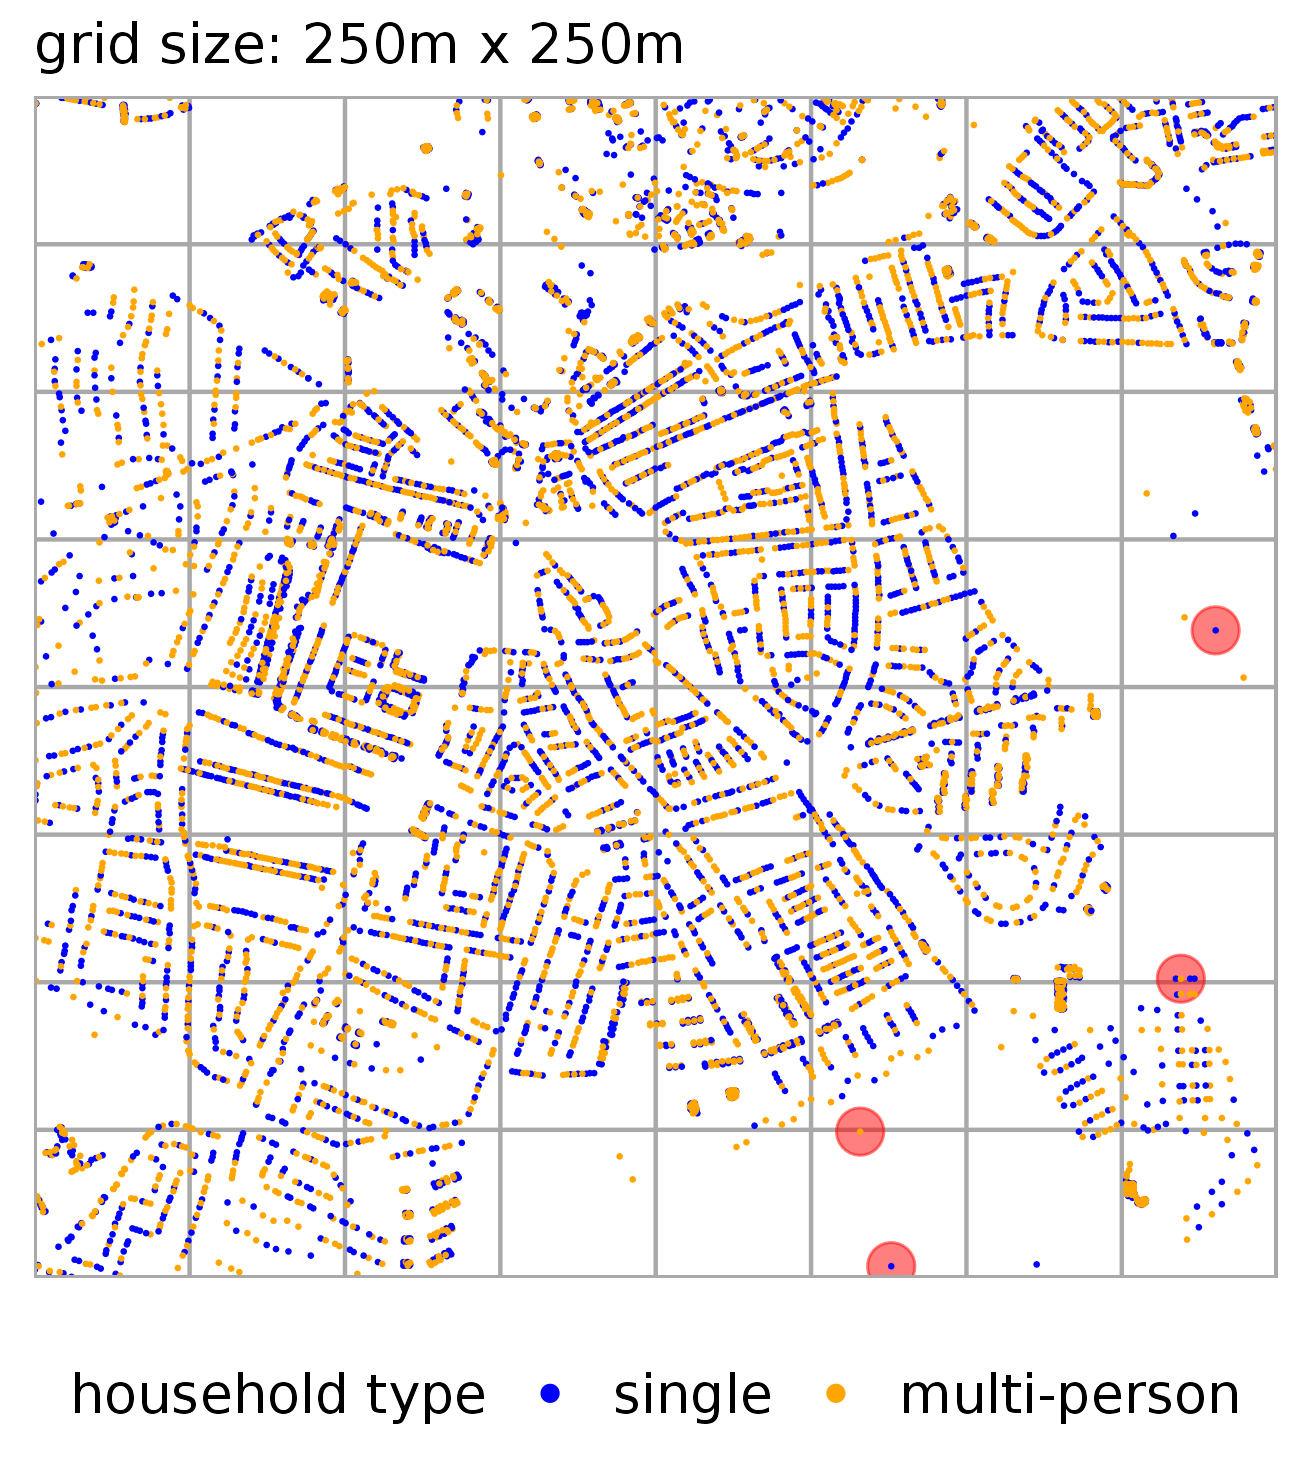
\includegraphics[width=0.495\linewidth]{figures/ExaMap_res1a.png}
    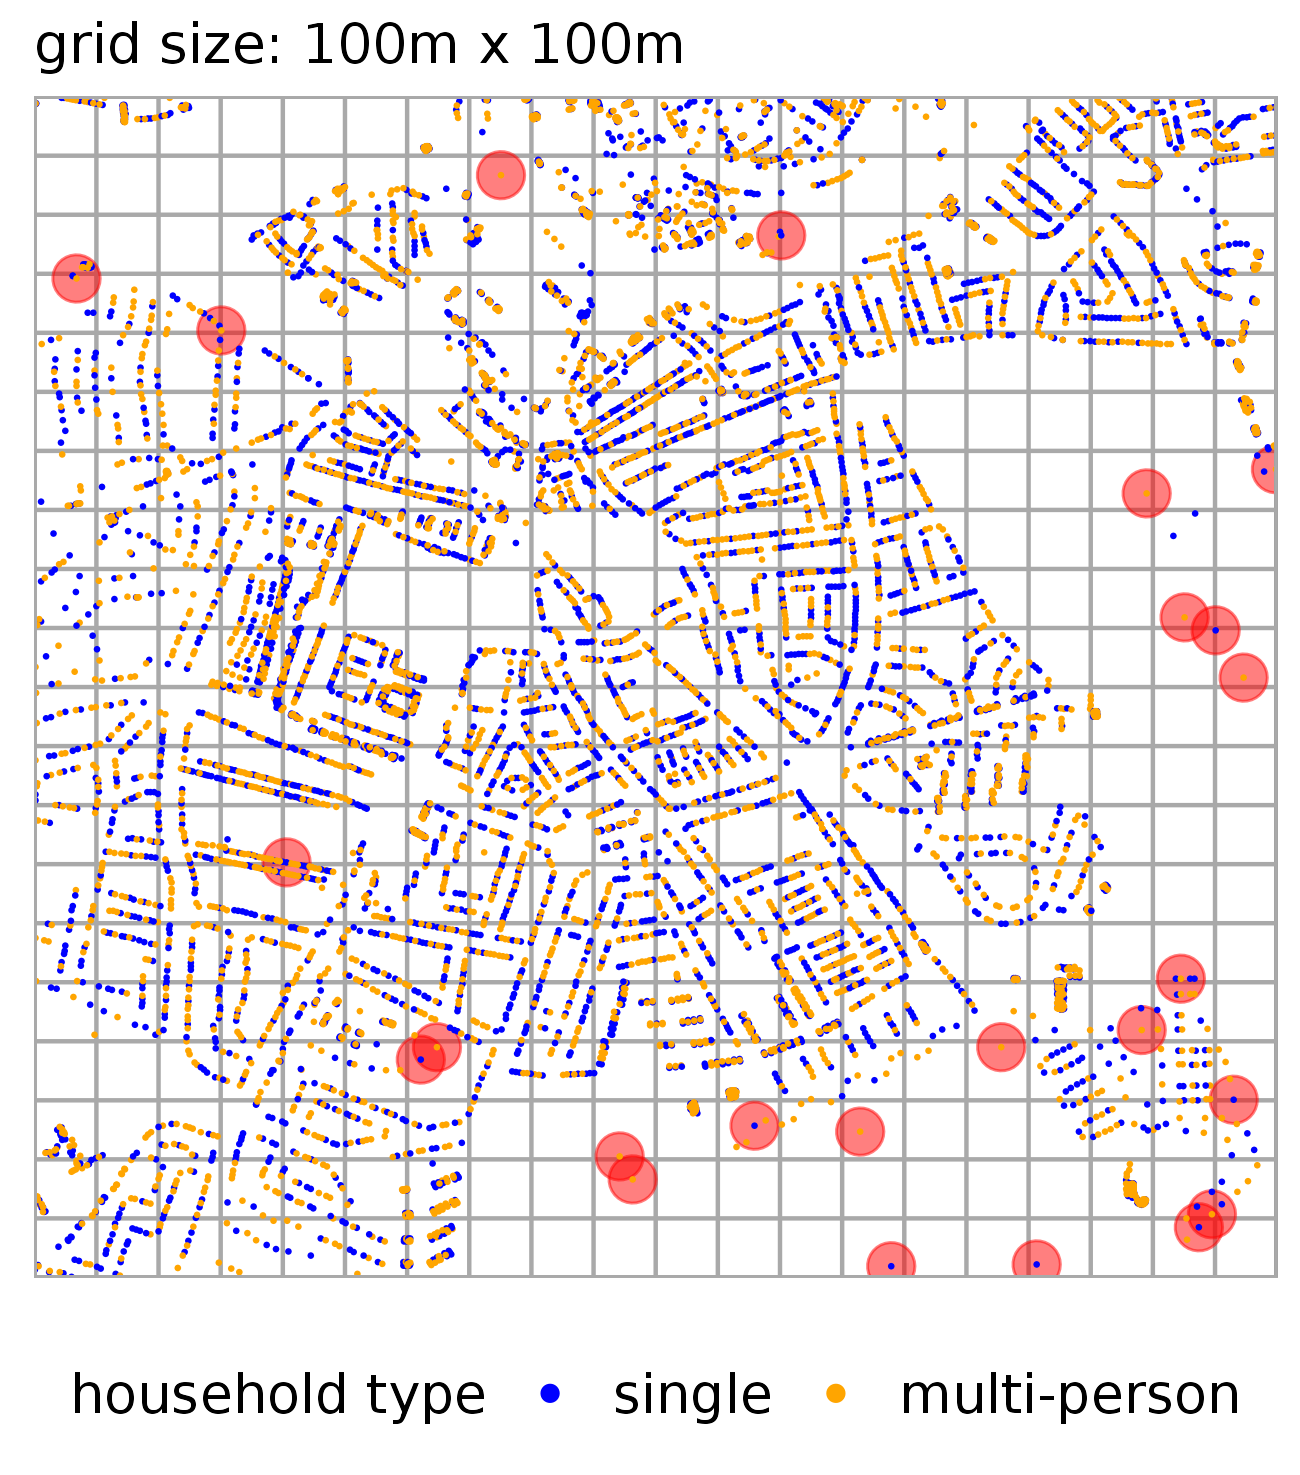
\includegraphics[width=0.495\linewidth]{figures/ExaMap_res1b.png}
    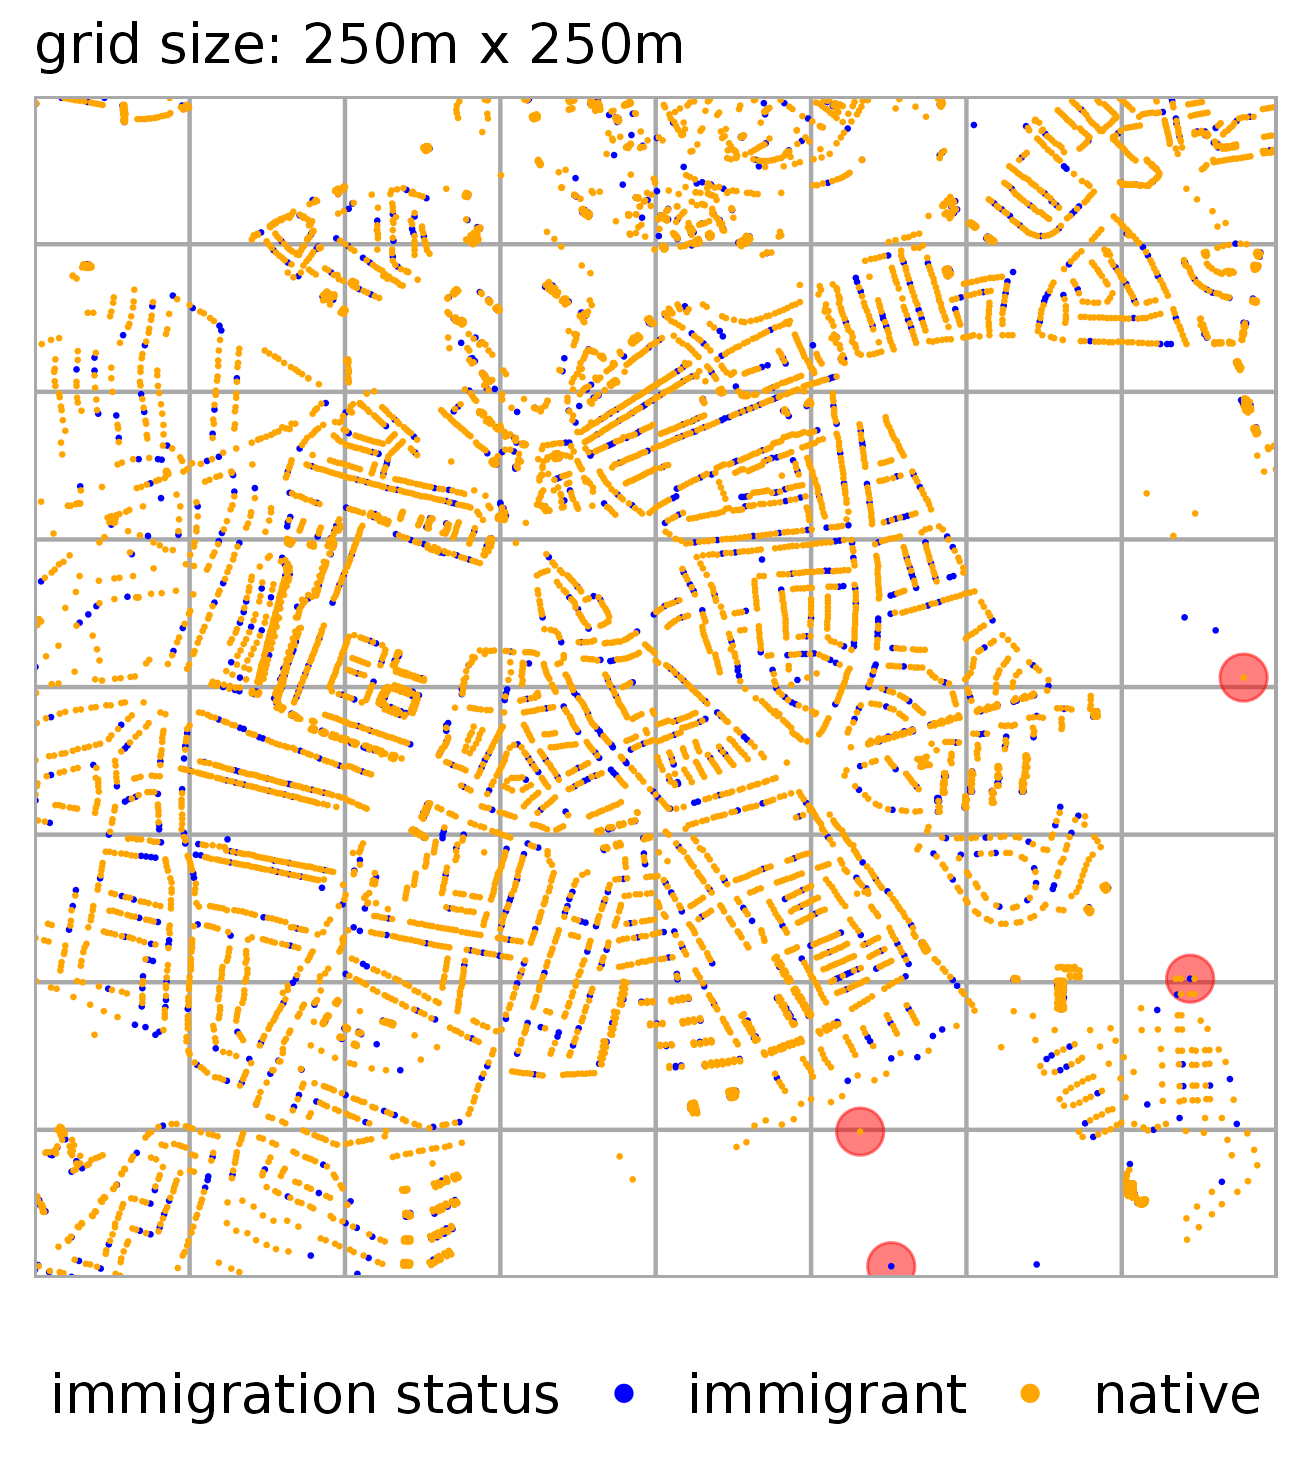
\includegraphics[width=0.495\linewidth]{figures/ExaMap_res2a.png}
    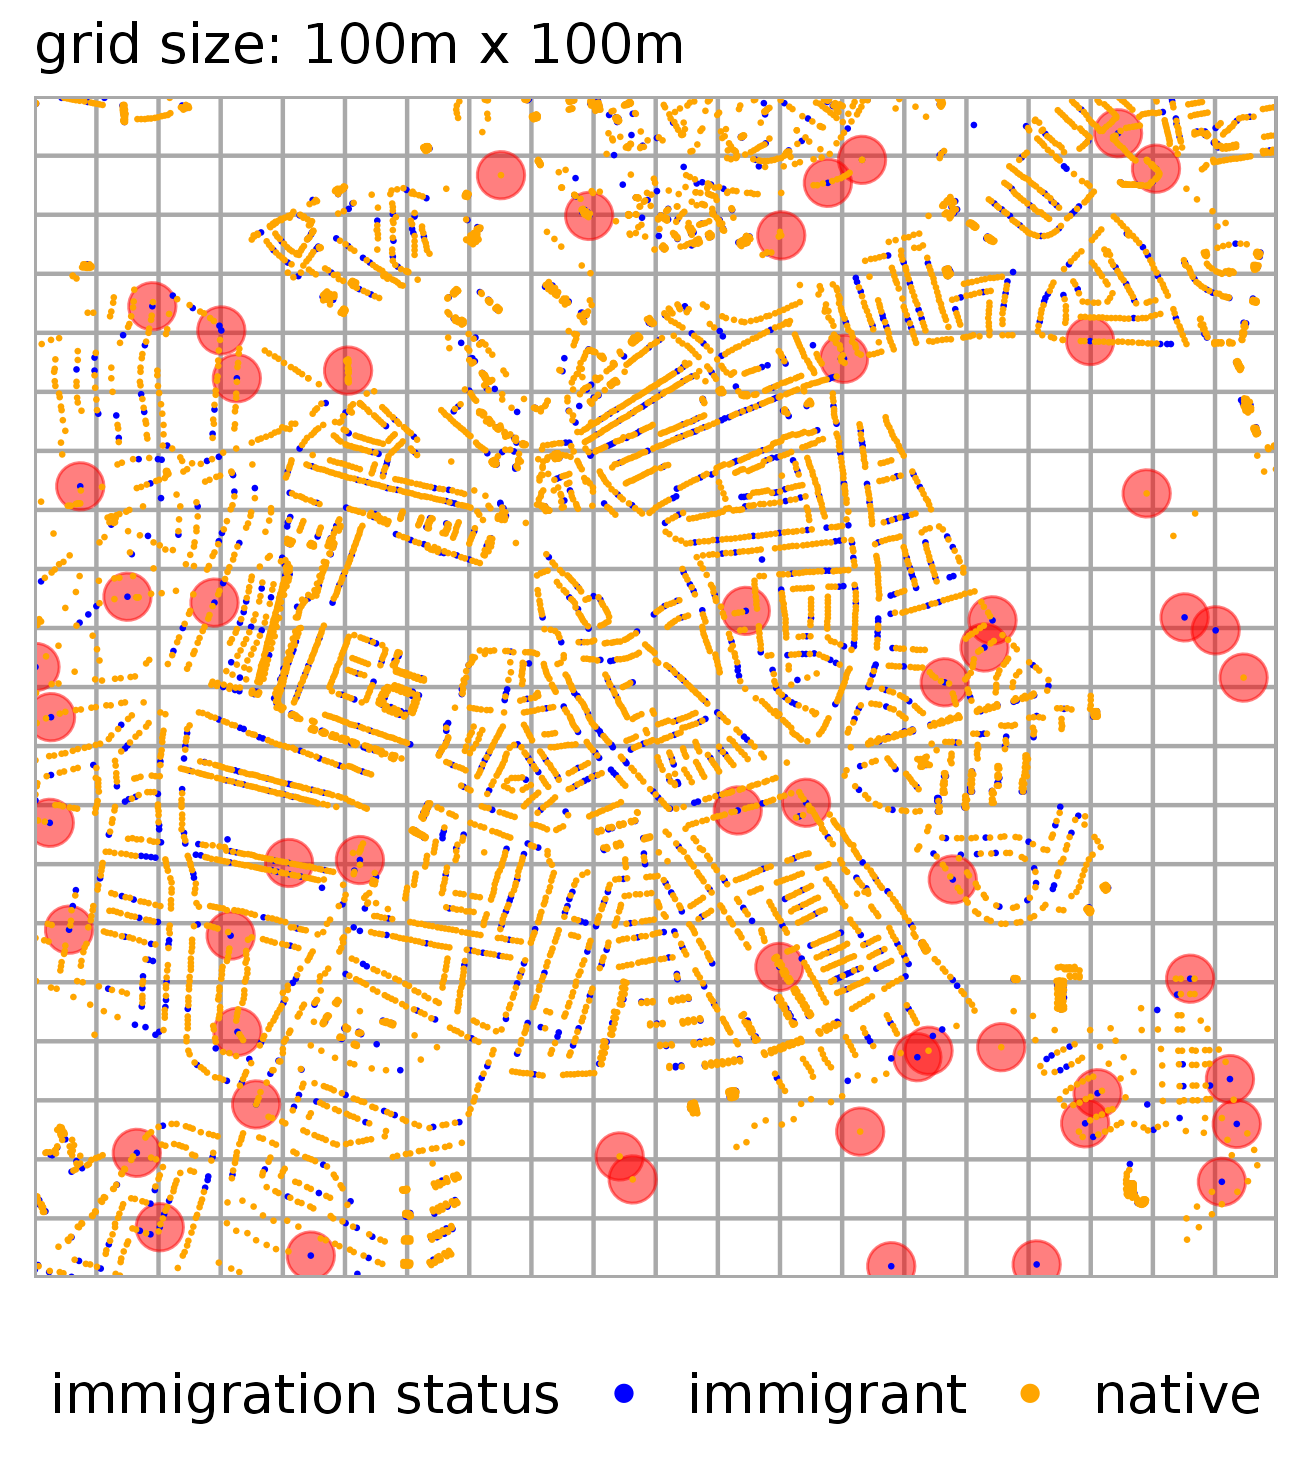
\includegraphics[width=0.495\linewidth]{figures/ExaMap_res2b.png}
    \caption{Fictitious maps of households by attribute `household type' (top) or `immigration status' (bottom), overlayed with geographic grid cells of size 250m $\times$ 250m (left) or 100m $\times$ 100m (right); marked in red are all households that would be uniquely identified by the cross-tabulation of grid cell and attribute.}
    \label{fig:ExaResMaps}
\end{figure}

The graph in Fig. \ref{fig:ExaResGraph} shows the number of aggregates that would only result in a single observation (count of 1) as a function of grid cell size. It illustrates that, generally speaking, \textit{the higher the level of detail in the geo-reference, the higher the expected risk of disclosure, especially for rare attributes}.\footnote{
    Note that we considered here attributes with only two categories. With more categories in the attribute, the issue would quickly be exacerbated further. The same is true when we add a third or fourth variable to the analysis. Incidentally, with a grid size of 100m $\times$ 100m, a 3-way aggregation of grid cell $\times$ household type $\times$ immigration status would leave 134 households identifiable, more than twice as many as in the most sensitive 2-way aggregation.
}
\begin{figure}
    \centering
    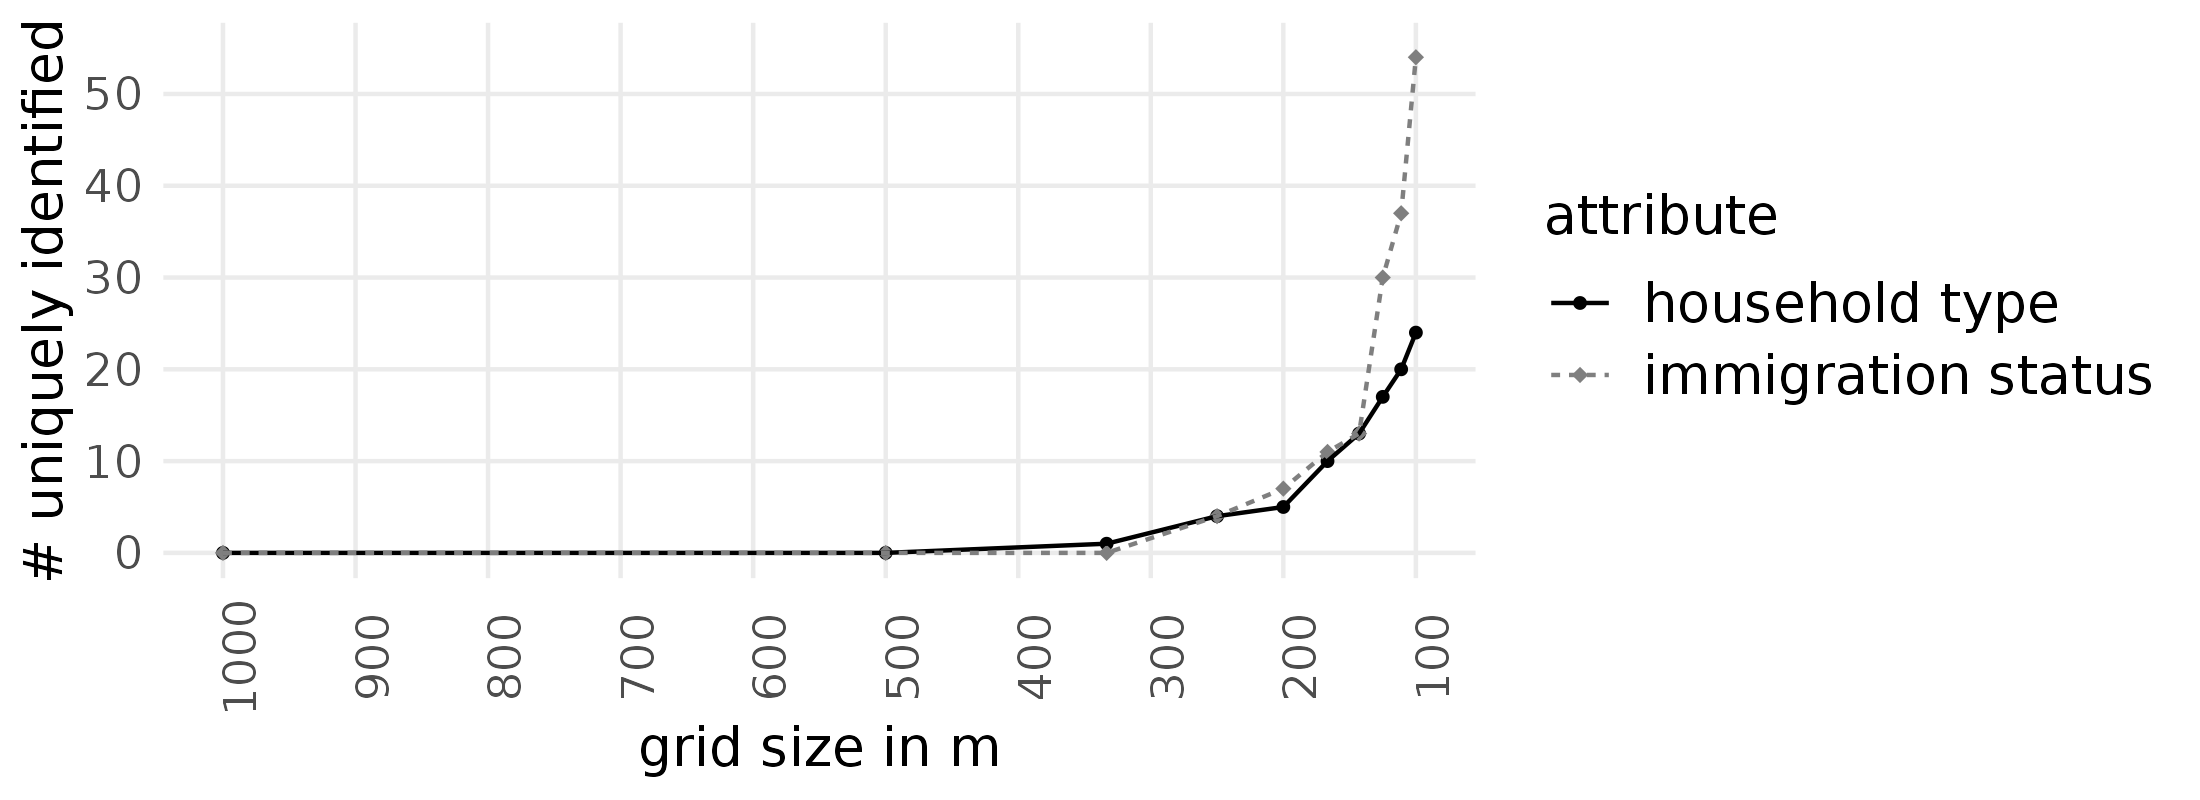
\includegraphics[width=\linewidth]{figures/ExaGraph_res2.png}
    \caption{No. of households from Fig. \ref{fig:ExaResMaps} uniquely identified by grid cell and attribute value as a function of cell size.}
    \label{fig:ExaResGraph}
\end{figure}

%\begin{figure}[H]
%    \centering
%    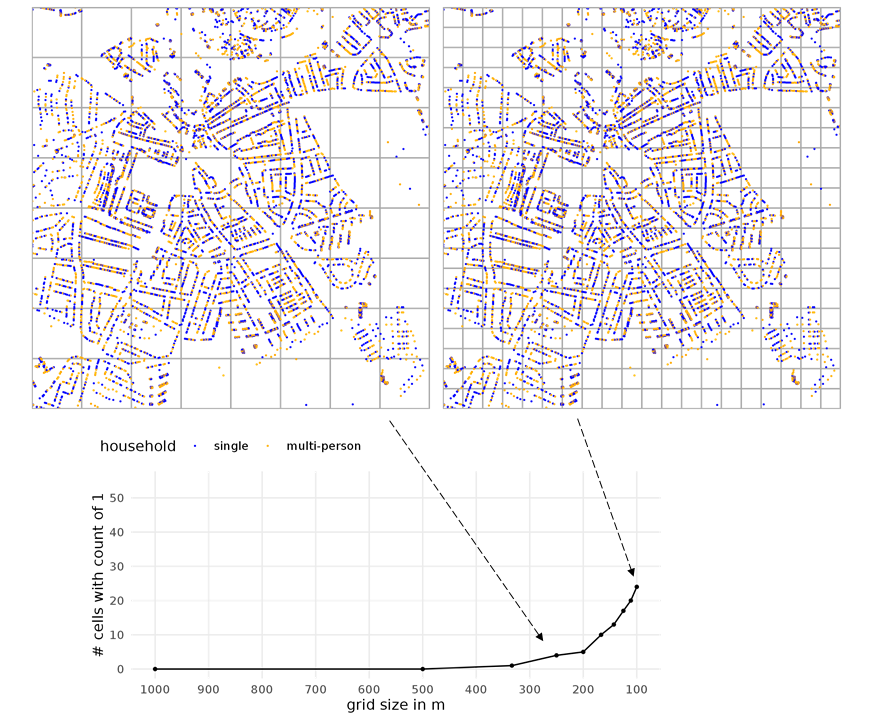
\includegraphics[width=\linewidth]{figures/ExaRes1.png}
%    \caption{Maps of households by type and grid cell (top); left: 250m $\times$ 250m grid, right: 100m $\times$ 100m grid; below: no. of households uniquely identified by grid cell and household type as a function of cell size.}
%    \label{fig:ExaRes1}
%\end{figure}

%\begin{figure}[H]
%    \centering
%    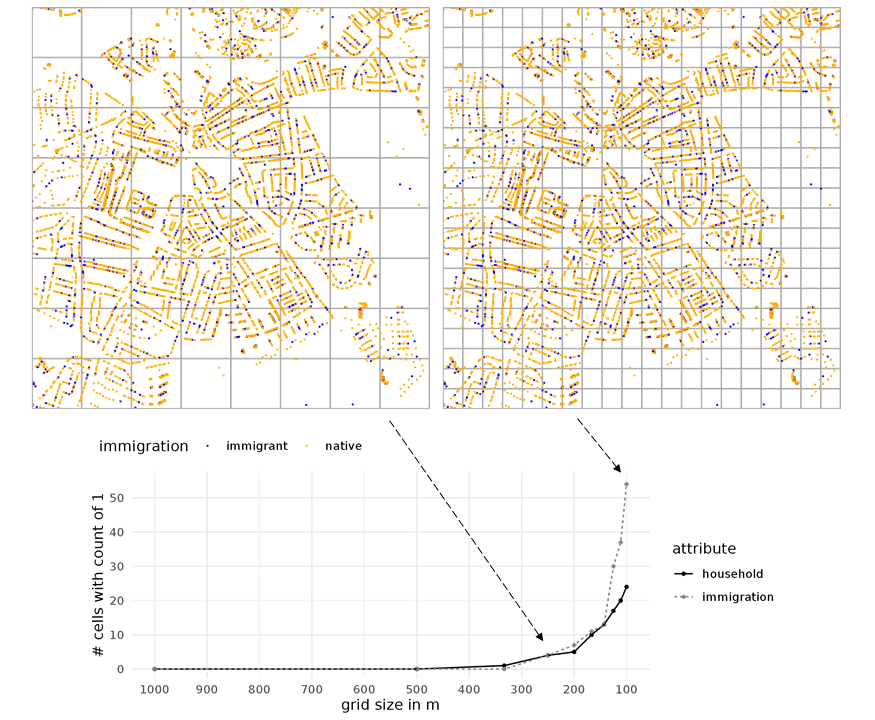
\includegraphics[width=\linewidth]{figures/ExaRes2.png}
%    \caption{Maps of households by immigration status and grid cell (top); left: 250m $\times$ 250m grid, right: 100m $\times$ 100m grid; below: no. of households uniquely identified by grid cell and immigration status as a function of cell size (graph from Fig. \ref{fig:ExaRes1} for reference).}
%    \label{fig:ExaRes2}
%\end{figure}

\subsection{The role of geographical characteristics of populations} \label{sec:ident_geochar}

\subsubsection{Population density and clustered versus disperse populations}

The (overall) population density is the total count of statistical units divided by the total size of the geographical space of interest. Generally speaking, the higher the population density, the more detailed the geo-reference can be, while still including enough units for each area and non-spatial attribute value to prevent disclosure problems. Likewise, for a given size of a geo-reference, the risk of disclosure tends to be higher in low-density compared to high-density regions. However, the total number of observations over a given geographical space can be a somewhat misleading indicator, since in reality population density is strongly heterogeneous. Therefore, one further needs to consider the local clustering characteristics of the population of interest.

\emph{Clustering} denotes the tendency of statistical units to crowd together in space. Consider the two populations of households mapped in Fig. \ref{fig:ExaDispClus} as dots. The one on the left sticks closely together, forming a heap or \emph{cluster}. The one on the right, on the other hand, disperses over the map much more consistently. Both patterns can be found in practice: the left one is typical for towns and cities, whereas the right one can sometimes be found in rural regions, for instance where households form farmsteads with surrounding arable land.
Clusters can provide a natural form of protection, as units blend together in dense centers, such as areas no. 6, 7, 10, and 11 in Fig. \ref{fig:ExaDispClus} (left). However, at the margins of settlements and in rural regions, where units are spaced more loosely, disclosure problems often arise. This is illustrated in Table \ref{tab:ExaDispClus}.

\begin{figure}[H]
    \centering
    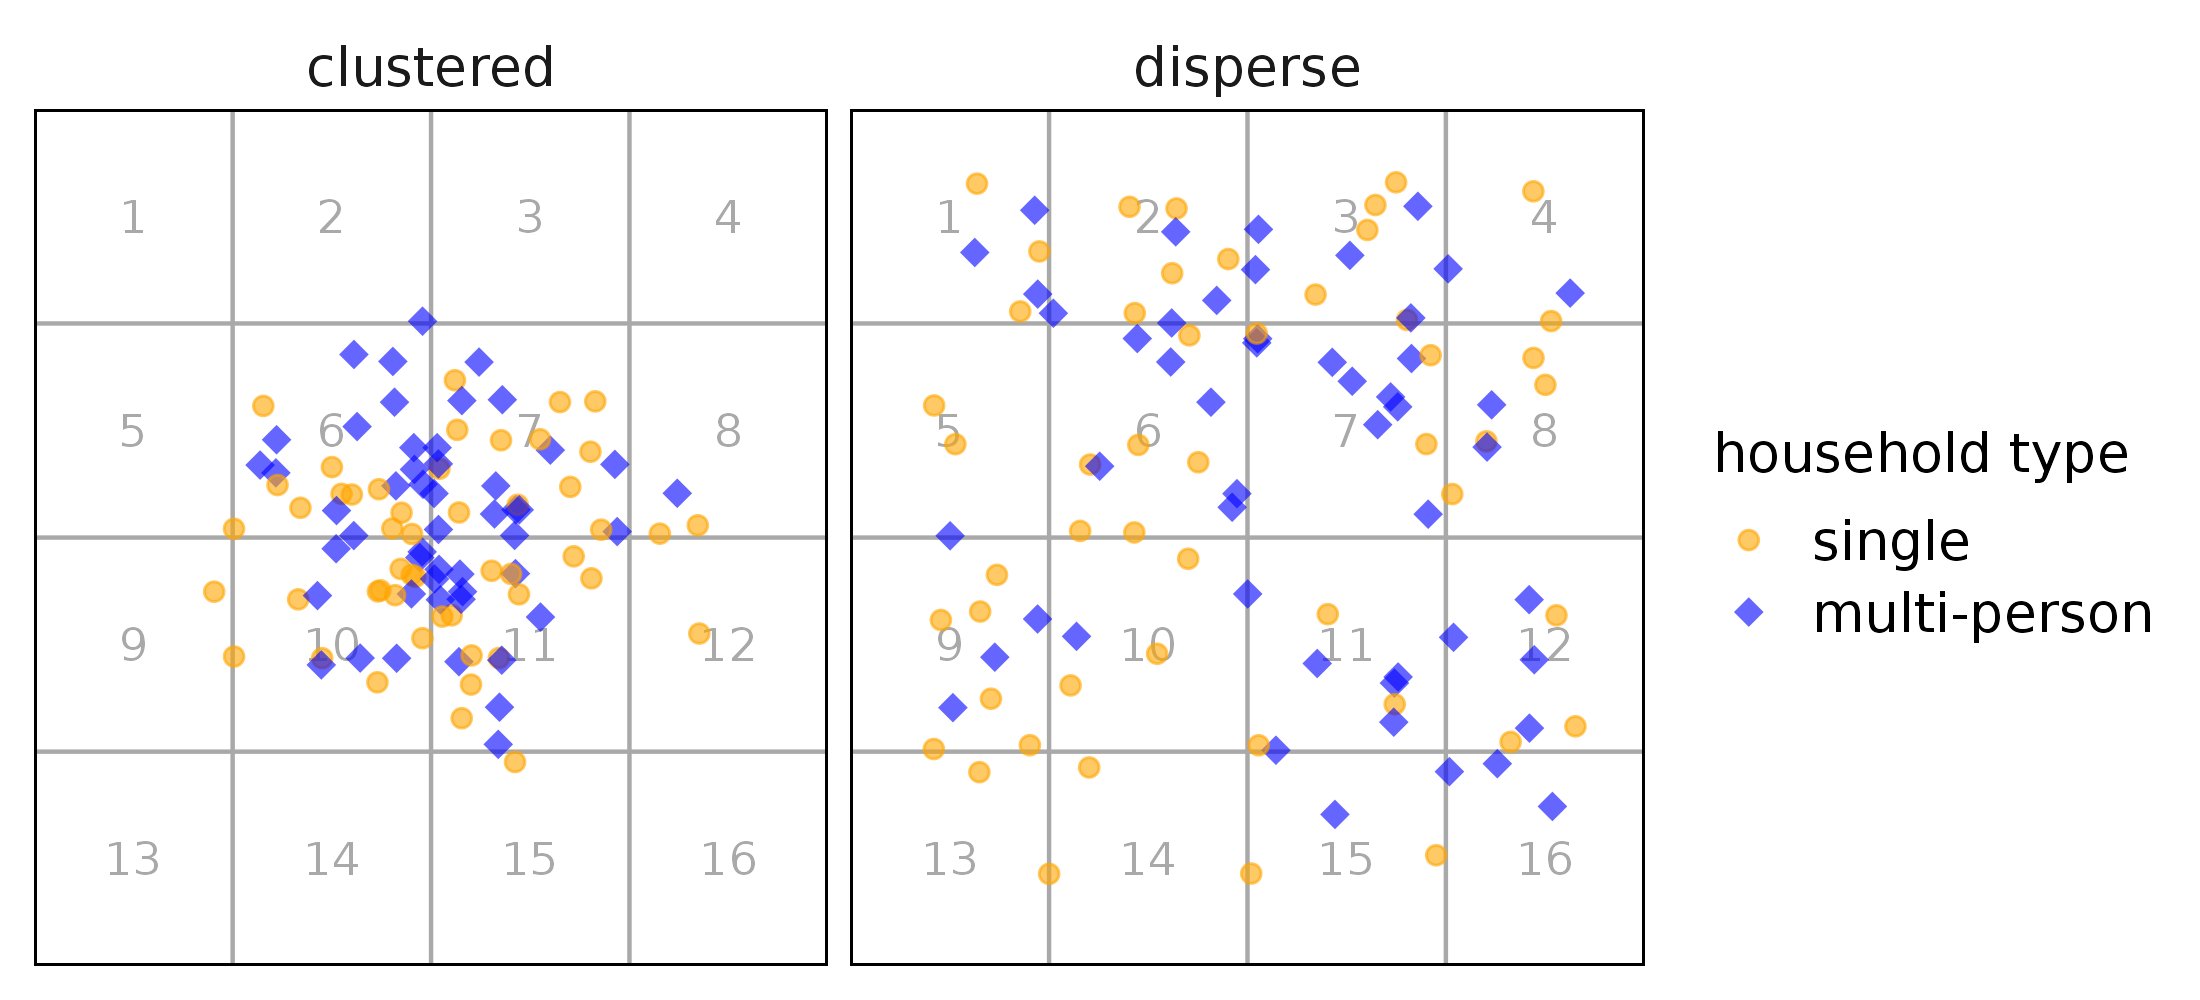
\includegraphics[width=\linewidth]{figures/ExaMap_clus_disp.png}
    \caption{Two artificial populations of the same size ($N = 100$), displaying different geographic characteristics: left clustered, right disperse; both are additionally classified by an attribute variable (household type); sub-areas of the map are numbered 1-16.}
    \label{fig:ExaDispClus}
\end{figure}

\begin{table}[H]
    \centering
    \begin{tabular}{|l|cc|c|  c  |l|cc|c|}
        \multicolumn{4}{c}{\emph{clustered}} & \multicolumn{1}{c}{} & \multicolumn{4}{c}{\emph{disperse}}\\[7pt]
        \cline{1-4} \cline{6-9}
        \multirow{2}{*}{area} & \multicolumn{2}{c|}{household type} & \multirow{2}{*}{total} & &
        \multirow{2}{*}{area} & \multicolumn{2}{c|}{household type} & \multirow{2}{*}{total}\\[5pt]
         & single & multi & & & & single & multi & \\
        \cline{1-4} \cline{6-9}
        1  & -  & -  & -  &  & 1  & \textcolor{blue}{3} & \textcolor{blue}{3} & 6  \\
        2  & -  & \textcolor{red}{1}  & \textcolor{red}{1}  &  & 2  & 5 & \textcolor{blue}{4} & 9  \\
        3  & -  & -  & -  &  & 3  & 5 & 5 & 10 \\
        4  & -  & -  & -  &  & 4  & \textcolor{red}{2} & \textcolor{red}{2} & \textcolor{blue}{4}  \\
        5  & -  & -  & -  &  & 5  & \textcolor{red}{2} & \textcolor{red}{1} & \textcolor{blue}{3}  \\
        6  & 11 & 13 & 24 &  & 6  & 6 & 6 & 12 \\
        7  & 12 & 15 & 27 &  & 7  & \textcolor{blue}{3} & 9 & 12 \\
        8  & \textcolor{red}{2}  & \textcolor{red}{1}  & \textcolor{blue}{3}  &  & 8  & \textcolor{blue}{4} & \textcolor{red}{2} & 6  \\
        9  & \textcolor{red}{1}  & -  & \textcolor{red}{1}  &  & 9  & 6 & \textcolor{blue}{3} & 9  \\
        10 & 11 & 8  & 19 &  & 10 & \textcolor{blue}{3} & \textcolor{red}{1} & \textcolor{blue}{4}  \\
        11 & 11 & 12 & 23 &  & 11 & \textcolor{blue}{3} & 6 & 9  \\
        12 & \textcolor{red}{1}  & -  & \textcolor{red}{1}  &  & 12 & \textcolor{blue}{3} & \textcolor{blue}{4} & 7  \\
        13 & -  & -  & -  &  & 13 & \textcolor{red}{1} & - & \textcolor{red}{1}  \\
        14 & -  & -  & -  &  & 14 & \textcolor{red}{2} & - & \textcolor{red}{2}  \\
        15 & \textcolor{red}{1}  & -  & \textcolor{red}{1}  &  & 15 & \textcolor{red}{2} & \textcolor{red}{1} & \textcolor{blue}{3}  \\
        16 & -  & -  & -  &  & 16 & - & \textcolor{blue}{3} & \textcolor{blue}{3}  \\
        \cline{1-4} \cline{6-9}
        \cline{1-4} \cline{6-9}
        total & 50 & 50 & 100 & & total & 50 & 50 & 100\\ 
        \cline{1-4} \cline{6-9}
    \end{tabular}
    \caption{Tabular representation of Fig. \ref{fig:ExaDispClus} data; cells in red are sensitive, when a minimum frequency rule of 3 is used, cells in blue are additionally sensitive, when a minimum frequency rule of 5 is used.}
    \label{tab:ExaDispClus}
\end{table}

%\begin{table}[H]
%    \centering
%    \begin{tabular}{|l|cc|c|  c  |l|cc|c|}
%        \multicolumn{4}{c}{\emph{clustered}} & \multicolumn{1}{c}{} & \multicolumn{4}{c}{\emph{disperse}}\\[7pt]
%        \cline{1-4} \cline{6-9}
%        \multirow{2}{*}{area} & \multicolumn{2}{c|}{household type} & \multirow{2}{*}{total} & &
%        \multirow{2}{*}{area} & \multicolumn{2}{c|}{household type} & \multirow{2}{*}{total}\\[5pt]
%         & single & multi & & & & single & multi & \\
%        \cline{1-4} \cline{6-9}
%        1  & -  & -  & -  &  & 1  & \textcolor{blue}{3} & \textcolor{blue}{3} & 6  \\
%        2  & -  & \cellcolor{lgrey}\textcolor{red}{1}  & \cellcolor{lgrey}\textcolor{red}{1}  &  & 2  & 5 & \textcolor{blue}{4} & 9  \\
%        3  & -  & -  & -  &  & 3  & 5 & 5 & 10 \\
%        4  & -  & -  & -  &  & 4  & \textcolor{red}{2} & \textcolor{red}{2} & \textcolor{blue}{4}  \\
%        5  & -  & -  & -  &  & 5  & \textcolor{red}{2} & \textcolor{red}{1} & \textcolor{blue}{3}  \\
%        6  & 11 & 13 & 24 &  & 6  & 6 & 6 & 12 \\
%        7  & 12 & 15 & 27 &  & 7  & \textcolor{blue}{3} & 9 & 12 \\
%        8  & \textcolor{red}{2}  & \textcolor{red}{1}  & \textcolor{blue}{3}  &  & 8  & \textcolor{blue}{4} & \textcolor{red}{2} & 6  \\
%        9  & \cellcolor{lgrey}\textcolor{red}{1}  & \cellcolor{lgrey}-  & \cellcolor{lgrey}\textcolor{red}{1}  &  & 9  & 6 & \textcolor{blue}{3} & 9  \\
%        10 & 11 & 8  & 19 &  & 10 & \textcolor{blue}{3} & \textcolor{red}{1} & \textcolor{blue}{4}  \\
%        11 & 11 & 12 & 23 &  & 11 & \textcolor{blue}{3} & 6 & 9  \\
%        12 & \cellcolor{lgrey}\textcolor{red}{1}  & \cellcolor{lgrey}-  & \cellcolor{lgrey}\textcolor{red}{1}  &  & 12 & \textcolor{blue}{3} & \textcolor{blue}{4} & 7  \\
%        13 & -  & -  & -  &  & 13 & \cellcolor{lgrey}\textcolor{red}{1} & \cellcolor{lgrey}- & \cellcolor{lgrey}\textcolor{red}{1}  \\
%        14 & -  & -  & -  &  & 14 & \cellcolor{lgrey}\textcolor{red}{2} & \cellcolor{lgrey}- & \cellcolor{lgrey}\textcolor{red}{2}  \\
%        15 & \cellcolor{lgrey}\textcolor{red}{1}  & \cellcolor{lgrey}-  & \cellcolor{lgrey}\textcolor{red}{1}  &  & 15 & \textcolor{red}{2} & \textcolor{red}{1} & \textcolor{blue}{3}  \\
%        16 & -  & -  & -  &  & 16 & \cellcolor{lgrey}- & \cellcolor{lgrey}\textcolor{blue}{3} & \cellcolor{lgrey}\textcolor{blue}{3}  \\
%        \cline{1-4} \cline{6-9}
%        \cline{1-4} \cline{6-9}
%        total & 50 & 50 & 100 & & total & 50 & 50 & 100\\ 
%        \cline{1-4} \cline{6-9}
%    \end{tabular}
%    \caption{Tabular representation of Fig. \ref{fig:ExaDispClus} data; cells in red are sensitive, when a minimum frequency rule of 3 is used, cells in blue are additionally sensitive, when a minimum frequency rule of 5 is used. Grey rows are vulnerable to attribute disclosure \citep[5.2]{HundepoolEtAl2024}.
%    }
%    \label{tab:ExaDispClus}
%\end{table}

Table \ref{tab:ExaDispClus} is the frequency table representation of Fig. \ref{fig:ExaDispClus}. It is derived by cross-tabulating the area identifier (1-16) with household type (single or multi-person). For risk assessment we assume a frequency rule (see section \ref{sec:risk_aggr_geosp}), where a table cell is considered unsafe, if it contains fewer units than a certain threshold (here: 3 or 5). 
When comparing the two tables side by side, it becomes clear that the level of protection a \emph{clustered} population provides varies widely: units in the dense center enjoy strong protection, whereas units at the margin can be unsafe. 
In the case of a \emph{disperse} population, the distribution of counts is much more even and hence the risk of small cell counts is more widespread.

\subsubsection{Attribute clustering and `sticky' populations}

Following \cite{ElliotEtAl1998}, the concept of a `sticky' population means the tendency of statistical units to form geographical clusters according to their attributes. For instance, suppose we assign to each household in a large area one of 5 categories, depending on where it stands on the income ladder (richest 20\%, next-richest 20\% etc., all the way to the poorest 20\%). If we now look at a smaller subregion, do we expect all categories to appear with equal frequency? This is usually not the case, as people of some income category are likely to live in neighborhoods with others of the same category.

Such a clustering tendency can be assumed for some, but not for all variables that may be potentially identifying. For example, while the category of household income may be clustered, this is often not the case (or only to a small degree) for variables like age group or gender.\footnote{
    `Sticky' populations may be seen an application of \emph{Tobler's Law}, variously known is the \emph{First Law of Geography}, a heuristic by which interaction (and hence often correlation in attributes) is stronger between things that are geographically close to one-another, rather than far apart. See e.g. \citet{Miller2004}.
}
There are two main implications for disclosure risk:
\begin{enumerate}
    \item For a sticky population, risk of \emph{identity disclosure} \cite[5.2]{HundepoolEtAl2024} tends to be smaller than for a non-sticky population. This is because attribute clustering decreases the variability of attributes within a region. Such lower variability in turn decreases the expected number of rare or unique attribute combinations \citep{GreenbergVoshell1990}. 
    \item At the same time - and for exactly the same reason - stickiness can increase the risk of \emph{attribute disclosure} \citep{BuronFontaine2018}. People with shared characteristics that require special protection (e.g. asylum status) also tend to cluster in space.
\end{enumerate}

By way of example, consider the two populations mapped in Fig. \ref{fig:ExaDispClus_sticky}. The placement is the same as in Fig. \ref{fig:ExaDispClus}, but the attribute variable is changed to show a clustering tendency. Table \ref{tab:ExaDispClus_sticky} is again the frequency table representation of Fig. \ref{fig:ExaDispClus_sticky} (tabulating household type by area).

\begin{figure}[H]
    \centering
    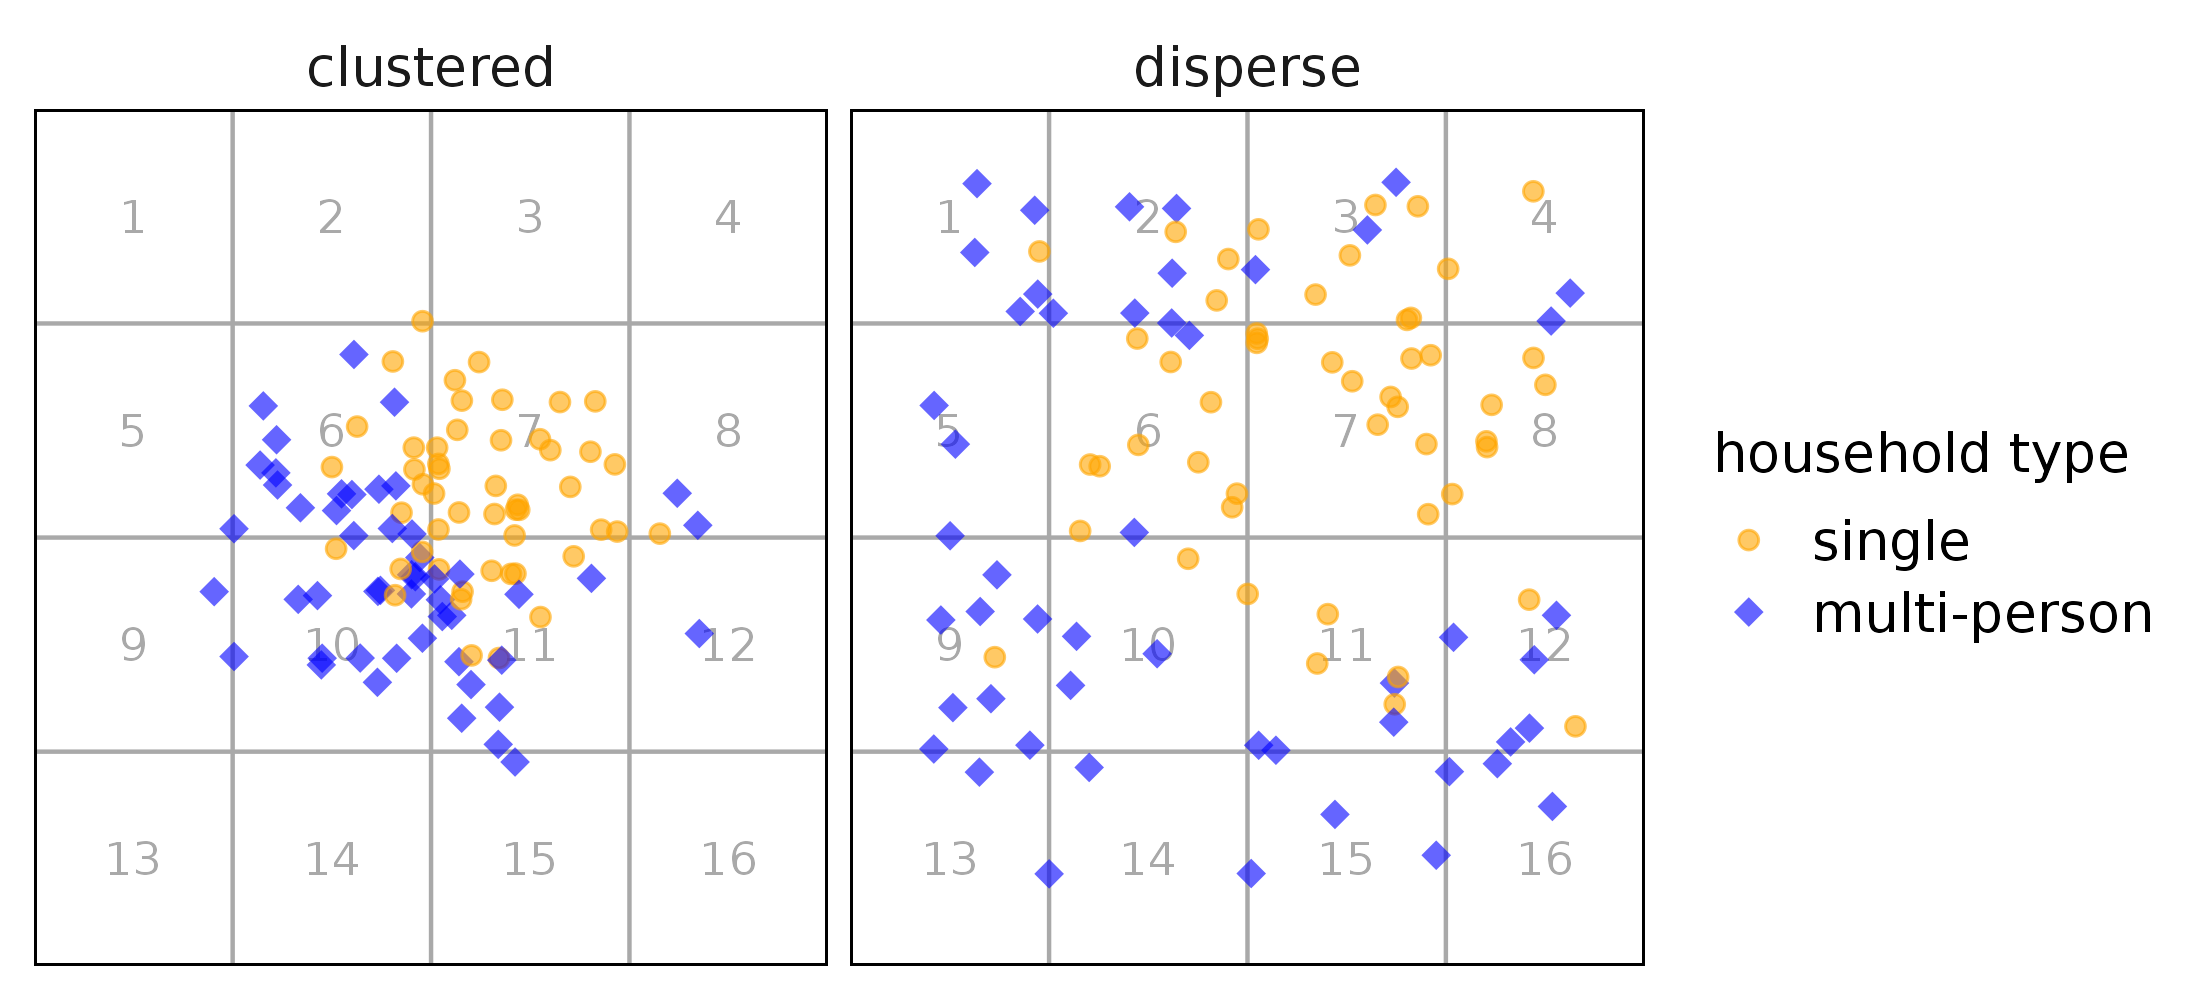
\includegraphics[width=\linewidth]{figures/ExaMap_clus_disp2.png}
    \caption{Alternative version of Fig. \ref{fig:ExaDispClus}, displaying attribute clustering. The sub-populations of single and multi-person households are `sticky', i.e. households with the same attribute tend to lump together spatially.}
    \label{fig:ExaDispClus_sticky}
\end{figure}

\begin{table}[H]
    \centering
    \begin{tabular}{|l|cc|c|  c  |l|cc|c|}
        \multicolumn{4}{c}{\emph{clustered}} & \multicolumn{1}{c}{} & \multicolumn{4}{c}{\emph{disperse}}\\[7pt]
        \cline{1-4} \cline{6-9}
        \multirow{2}{*}{area} & \multicolumn{2}{c|}{household type} & \multirow{2}{*}{total} & &
        \multirow{2}{*}{area} & \multicolumn{2}{c|}{household type} & \multirow{2}{*}{total}\\[5pt]
         & single & multi & & & & single & multi & \\
        \cline{1-4} \cline{6-9}
        1  & -  & -  & - &  & 1  & \textcolor{red}{1}  & 5 & 6  \\
        2  & \cellcolor{lgrey}\textcolor{red}{1}  & \cellcolor{lgrey}- & \cellcolor{lgrey}\textcolor{red}{1} &  & 2  & \textcolor{blue}{3}  & 6 & 9  \\
        3  & -  & -  & -  &  & 3  & 7  & \textcolor{blue}{3} & 10 \\
        4  & -  & -  & -  &  & 4  & \textcolor{red}{2}  & \textcolor{red}{2} & \textcolor{blue}{4}  \\
        5  & -  & -  & -  &  & 5  & \cellcolor{lgrey}-  & \cellcolor{lgrey}\textcolor{blue}{3} & \cellcolor{lgrey}\textcolor{blue}{3}  \\
        6  & 7  & 17 & 24 &  & 6  & 10 & \textcolor{red}{2} & 12 \\
        7  & \cellcolor{lgrey}27 & \cellcolor{lgrey}-  & \cellcolor{lgrey}27 &  & 7  & \cellcolor{lgrey}12 & \cellcolor{lgrey}- & \cellcolor{lgrey}12 \\
        8  & \textcolor{red}{1}  & \textcolor{red}{2}  & 3  &  & 8  & \cellcolor{lgrey}6  & \cellcolor{lgrey}- & \cellcolor{lgrey}6  \\
        9  & \cellcolor{lgrey}- & \cellcolor{lgrey}\textcolor{red}{1}  & \cellcolor{lgrey}\textcolor{red}{1}  &  & 9  & \textcolor{red}{1}  & 8 & 9  \\
        10 & \textcolor{blue}{4}  & 15 & 19 &  & 10 & \textcolor{red}{1}  & \textcolor{blue}{3} & \textcolor{blue}{4}  \\
        11 & 10 & 13 & 23 &  & 11 & 5  & \textcolor{blue}{4} & 9  \\
        12 & \cellcolor{lgrey}-  & \cellcolor{lgrey}\textcolor{red}{1}  & \cellcolor{lgrey}\textcolor{red}{1}  &  & 12 & \textcolor{red}{2}  & 5 & 7  \\
        13 & -  & -  & -  &  & 13 & \cellcolor{lgrey}-  & \cellcolor{lgrey}\textcolor{red}{1} & \cellcolor{lgrey}\textcolor{red}{1}  \\
        14 & -  & -  & -  &  & 14 & \cellcolor{lgrey}-  & \cellcolor{lgrey}\textcolor{red}{2} & \cellcolor{lgrey}\textcolor{red}{2}  \\
        15 & \cellcolor{lgrey}-  & \cellcolor{lgrey}\textcolor{red}{1}  & \cellcolor{lgrey}\textcolor{red}{1}  &  & 15 & \cellcolor{lgrey}-  & \cellcolor{lgrey}\textcolor{blue}{3} & \cellcolor{lgrey}\textcolor{blue}{3}  \\
        16 & -  & -  & -  &  & 16 & \cellcolor{lgrey}-  & \cellcolor{lgrey}\textcolor{blue}{3} & \cellcolor{lgrey}\textcolor{blue}{3}  \\
        \cline{1-4} \cline{6-9}
        \cline{1-4} \cline{6-9}
        total & 50 & 50 & 100 & & total & 50 & 50 & 100\\ 
        \cline{1-4} \cline{6-9}
    \end{tabular}
    \caption{Tabular representation of Fig. \ref{fig:ExaDispClus_sticky} data; cells in red are sensitive, when a minimum frequency rule of 3 is used, cells in blue are additionally sensitive, when a minimum frequency rule of 5 is used. Grey rows are vulnerable to attribute disclosure \citep[5.2]{HundepoolEtAl2024}.}
    \label{tab:ExaDispClus_sticky}
\end{table}

Compare Table \ref{tab:ExaDispClus_sticky} to Table \ref{tab:ExaDispClus}. For the clustered population, the switch to sticky populations did not change the number of table cells that fall below the frequency threshold. However, 31 units are now at risk of (group) attribute disclosure. Most notably, it is disclosed that whenever a household is located in area 7, it is a single person household. The corresponding number of units at risk of attribute disclosure in Table \ref{tab:ExaDispClus} (left) was 4.
Comparing the situation for the disperse population, we can see that the number of small cells that may pose a risk of identity disclosure is slightly lower (11 vs. 12 for the threshold of 3 and 12 vs. 16 for the threshold of 5). The number of units at risk of attribute disclosure has risen from 6 to 30.\\

In general, a clustering tendency for identifying variables can be helpful for avoiding disclosure, as it will tend to reduce the likelihood of rare attribute combinations. A clustering tendency for sensitive attributes, for which attribute disclosure is to be avoided, can be a challenge.

\section{Outputs based on geo-referenced data}

Geo-referenced data can be the basis for a variety of outputs. \emph{Microdata files} and \emph{aggregate tables} 
%(of frequencies or magnitudes) 
are the classical products of statistical offices.
%; see \citet[~p.7]{HundepoolEtAl2010}. 
With the inclusion of the spatial domain, detailed \emph{thematic maps} are added, which can be static (for print) or interactive (for digital publication). Maps often add analytical value over mere tabulations of spatial data; see, for instance, \citet{Waller2024}.
Fig. \ref{fig:rep_map} shows people aged 65 or above in a rural region, geo-referenced to grid cells of size 1km $\times$ 1km. Tables \ref{tab:rep_tab} and \ref{tab:rep_micro} present the same ground truth as alternative representations, once as frequency table and once as microdata table.

Typically all these outputs need to be protected and if one and the same data is used for two or all three types, it would be best if the protection is consistent across them. This is facilitated by an underlying equivalence: Fig. \ref{fig:rep_map} is a visualization of table \ref{tab:rep_tab}, which in turn tabulates micro data table \ref{tab:rep_micro}.
Some methods of disclosure control, like the Cell Key Method (see section \ref{sec:ckm}), therefore protect the map by protecting the table. Others, like Targeted record swapping (see section \ref{sec:trs}), act on the micro data to protect the tables and maps derived from it. Still others, like spatial smoothing (see section \ref{sec:methods_smooth}), consider the map an output product in its own right and aim to protect it specifically.

\newpage

% Map centered around ca. lat 6.33, lon 51.63 in Web Mercator (R package mapView); betw. Kervenheim and Sonsbeck, SE of Kleve (NW), Germany, near the border to Netherlands; grid definition in ETRS89 LAEA
\begin{figure}[H]
    \centering
    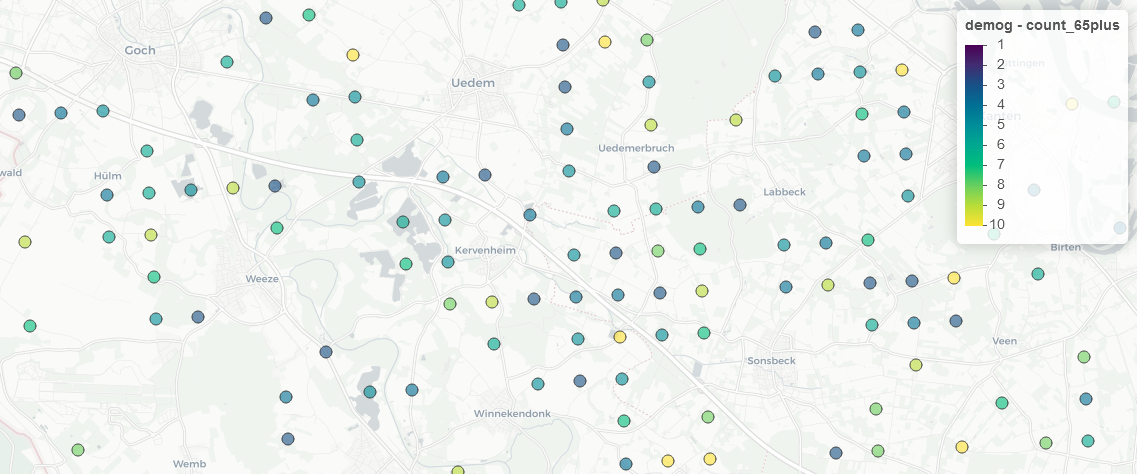
\includegraphics[width=\linewidth]{figures/rep_map.png}
    \caption{\emph{Map} representation of geo-referenced data (no. of inhabitants aged 65+ in 1km$^2$ grid cells); each colored marker equates to a table cell in aggregate table \ref{tab:rep_tab} and a block of entries in microdata table \ref{tab:rep_micro}.}
    \label{fig:rep_map}
\end{figure}

\begin{table}[H]
    \centering
    \begin{tabular}{c | c c c c c}
         \multirow{2}*{Northing} & \multicolumn{4}{c}{Easting} &\\
         & E:4065 & E:4066 & E:4067 & E:4068 & \ldots \\
         \hline
         N:3176 & - & 6 & 3 & 4 & \multirow{3}*{$\cdots$}\\
         N:3175 & 5 & 3 & 8 & 7 &\\
         N:3174 & 4 & 4 & 3 & 9 &\\
         \vdots & \multicolumn{4}{c}{\vdots} & $\ddots$
    \end{tabular}
    \caption{\emph{Table} representation of geo-referenced data (no. of inhabitants aged 65+ in 1km$^2$ grid cells), each table cell equates to a colored marker in map Fig. \ref{fig:rep_map} and a block of entries in microdata table \ref{tab:rep_micro}.}
    \label{tab:rep_tab}
\end{table}

\begin{table}[H]
    \centering
    \begin{tabular}{c c c}
         unit ID & grid cell ID & age group \\
         \hline
         1 & N:3176 E:4066 & 65+ \\
         2 & N:3176 E:4066 & 65+ \\
         3 & N:3176 E:4066 & 65+ \\
         4 & N:3176 E:4066 & 65+ \\
         5 & N:3176 E:4066 & 65+ \\
         6 & N:3176 E:4066 & 65+ \\
         7 & N:3176 E:4067 & 65+ \\
         8 & N:3176 E:4067 & 65+ \\
         9 & N:3176 E:4067 & 65+ \\
         \multicolumn{3}{c}{$\vdots$}
    \end{tabular}
    \caption{\emph{Microdata} representation of geo-referenced data (inhabitants aged 65+ in 1km$^2$ grid cells); each block of entries with same grid cell ID equates to  a colored marker in map Fig. \ref{fig:rep_map} and a table cell in aggregate table \ref{tab:rep_tab}.}
    \label{tab:rep_micro}
\end{table}

